
\documentclass[a4paper,USenglish,cleveref, autoref, thm-restate, anonymous]{lipics-v2021}
%This is a template for producing LIPIcs articles. 
%See lipics-v2021-authors-guidelines.pdf for further information.
%for A4 paper format use option "a4paper", for US-letter use option "letterpaper"
%for british hyphenation rules use option "UKenglish", for american hyphenation rules use option "USenglish"
%for section-numbered lemmas etc., use "numberwithinsect"
%for enabling cleveref support, use "cleveref"
%for enabling autoref support, use "autoref"
%for anonymousing the authors (e.g. for double-blind review), add "anonymous"
%for enabling thm-restate support, use "thm-restate"
%for enabling a two-column layout for the author/affilation part (only applicable for > 6 authors), use "authorcolumns"
%for producing a PDF according the PDF/A standard, add "pdfa"

\pdfoutput=1 %uncomment to ensure pdflatex processing (mandatatory e.g. to submit to arXiv)
\hideLIPIcs  %uncomment to remove references to LIPIcs series (logo, DOI, ...), e.g. when preparing a pre-final version to be uploaded to arXiv or another public repository

%\graphicspath{{./graphics/}}%helpful if your graphic files are in another directory

\bibliographystyle{plainurl}% the mandatory bibstyle

\title{Cross-Domain Integrity with Controller Labels and Endorsement}% mandatory

%\titlerunning{Dummy short title} %TODO optional, please use if title is longer than one line

\author{Isaac Sheff}{Heliax, Buffalo, USA \and \url{https://isaacsheff.com} }{isaac@heliax.dev}{https://orcid.org/0000-0002-1825-0097}{[(Optional) author-specific funding acknowledgements]}%TODO mandatory, please use full name; only 1 author per \author macro; first two parameters are mandatory, other parameters can be empty. Please provide at least the name of the affiliation and the country. The full address is optional. Use additional curly braces to indicate the correct name splitting when the last name consists of multiple name parts.

% \author{Christopher W. Goes}{Heliax, Berlin, Germany}{cwgoes@heliax.dev}{[orcid]}{[funding]}

\authorrunning{I. Sheff \& C. W. Goes} %TODO mandatory. First: Use abbreviated first/middle names. Second (only in severe cases): Use first author plus 'et al.'

\Copyright{Isaac Sheff and Christpher Goes} %TODO mandatory, please use full first names. LIPIcs license is "CC-BY";  http://creativecommons.org/licenses/by/3.0/

\ccsdesc[100]{\textcolor{red}{Replace ccsdesc macro with valid one}} %TODO mandatory: Please choose ACM 2012 classifications from https://dl.acm.org/ccs/ccs_flat.cfm 

\keywords{Dummy keyword} %TODO mandatory; please add comma-separated list of keywords

\category{} %optional, e.g. invited paper

\relatedversion{} %optional, e.g. full version hosted on arXiv, HAL, or other respository/website
%\relatedversiondetails[linktext={opt. text shown instead of the URL}, cite=DBLP:books/mk/GrayR93]{Classification (e.g. Full Version, Extended Version, Previous Version}{URL to related version} %linktext and cite are optional

%\supplement{}%optional, e.g. related research data, source code, ... hosted on a repository like zenodo, figshare, GitHub, ...
%\supplementdetails[linktext={opt. text shown instead of the URL}, cite=DBLP:books/mk/GrayR93, subcategory={Description, Subcategory}, swhid={Software Heritage Identifier}]{General Classification (e.g. Software, Dataset, Model, ...)}{URL to related version} %linktext, cite, and subcategory are optional

%\funding{(Optional) general funding statement \dots}%optional, to capture a funding statement, which applies to all authors. Please enter author specific funding statements as fifth argument of the \author macro.

\acknowledgements{}%optional

%\nolinenumbers %uncomment to disable line numbering



%Editor-only macros:: begin (do not touch as author)%%%%%%%%%%%%%%%%%%%%%%%%%%%%%%%%%%
% \EventEditors{John Q. Open and Joan R. Access}
% \EventNoEds{2}
% \EventLongTitle{42nd Conference on Very Important Topics (CVIT 2016)}
% \EventShortTitle{CVIT 2016}
% \EventAcronym{CVIT}
% \EventYear{2016}
% \EventDate{December 24--27, 2016}
% \EventLocation{Little Whinging, United Kingdom}
% \EventLogo{}
% \SeriesVolume{42}
% \ArticleNo{23}
%%%%%%%%%%%%%%%%%%%%%%%%%%%%%%%%%%%%%%%%%%%%%%%%%%%%%%


% Non-template imports
\usepackage{tikz}
\usepackage{subcaption}

% Non-template MACROS
\newcommand{\N}{\mathbb{N}}
\newcommand{\abs}[1]{\left|{#1}\right|}
\newcommand{\p}[1]{{\ensuremath{\left({{#1}}\right)}}}
\newcommand{\cb}[1]{{\left\{{{#1}}\right\}}}
\newcommand{\sqb}[1]{{\left[{{#1}}\right]}}
\newcommand{\an}[1]{{\left\langle{{#1}}\right\rangle}}
\newcommand{\ceil}[1]{{\ensuremath{\left\lceil{{#1}}\right\rceil}}}
\newcommand{\bb}[1]{{\left\llbracket{{#1}}\right\rrbracket}}
\newcommand{\tb}[1]{{\textrm{\textbf{{#1}}}}}
\newcommand{\ti}[1]{{\emph{{#1}}}}
\newcommand{\tallpipe}[2]{%
  {%
    \ensuremath{%
      \begin{array}{@{}r|l@{}}%
        {{#1}}&{{#2}}%
      \end{array}%
    }%
  }%
}
\newcommand{\join}{\mathbin{\sqcup}}
\newcommand{\meet}{{\ensuremath{\sqcap}}}
\newcommand{\eqdef}{\ensuremath{\overset{\mathrm{def}}{=}}}

\newcommand{\resources}{{\ensuremath{\mathcal R}}}


\newcommand{\colort}[2]{{\color{#1}{#2}}}
\newcommand{\red}[1]{\colort{red}{#1}}
\newcommand{\blue}[1]{\colort{blue}{#1}}
\newcommand{\green}[1]{{\colort{DarkGreen}{#1}}}
\newcommand{\purple}[1]{{\colort{purple}{#1}}}
\newcommand{\orange}[1]{{\colort{orange}{#1}}}
\newcommand{\gray}[1]{{\colort{gray}{#1}}}

\newcommand{\basecoin}{\blue{BaseCoin}}
\newcommand{\basechain}{\blue{BaseChain}}
\newcommand{\sidechain}{\purple{SideChain}}

\newcommand{\JuvixCore}{\ensuremath{\mathsf{JuvixCore}}}
\newcommand{\Geb}{\ensuremath{\mathsf{Geb}\,}}
\newcommand{\Juvix}{\ensuremath{\mathsf{Juvix}}}
\newcommand{\VampIR}{\ensuremath{\mathsf{VampIR}}}
\newcommand{\LambdaIR}{\ensuremath{\mathsf{Lambda}}}




\begin{document}

\maketitle

%TODO mandatory: add short abstract of the document
\begin{abstract}
In distributed systems, mutable digital objects typically require some state machine to decide on their definitive current state.
This state machine can be replicated to enhance availability and fault tolerance.
We call the authoritative state machine of a digital object its \emph{controller}.
Typical examples of controllers defining objects include a database storing a record, or a blockchain storing the current state of a smart contract.
Without some kind of controller, different parties may have contradictory notions of what the state is, and no way to reconcile them.
In a distributed system, some controllers may be \emph{Byzantine}, and make duplicitous or incoherent statements about state. 

Here we design rules and procedures for a multi-state-machine ecosystem, featuring digital objects, or \emph{resources}, with application-defined state-dependent rules for how they can be updated. 
% ICS: not relevant to this paper: Resources can even be \emph{shielded}, where the and state of the resource is hidden from the controller itself. 
Each controller can express an authoritative state, including authoritative resource states. 
Each resource is also labeled with a controller identifier, whose state is definitive for this resource. 
Resources can transfer between controllers, and updates can depend on multiple resources, so resource labels also express a \emph{dependency graph} detailing which controllers, if they were Byzantine, may have corrupted this resource.
In a sense, these labels represent a distributed \emph{taint tracking} or \emph{dynamic information flow control} solution.
One challenge is avoiding size explosion in this dependency graph: we enable removing unnecessary parts of history when, say, a resource transfers from $A$ to $B$ and back to $A$ again.
In information flow control terms, these operations require \emph{endorsement}.
Our resource controller operations generalize a number of techniques used in blockchain settings.
We define rules and procedures for creating, updating, transferring, and tracking the state of labeled resources, and prove that our rules maintain safety properties including \emph{causal resource history} and \emph{consistent controller labels}.
\end{abstract}

\section{Introduction}
Distributed platform interoperability is crucial to improve cost, usability, adoption, and even security. 
When applications must share a state machine (or, more generally, \emph{controller}) to interact, there is an incentive to push all applications onto one controller trustworthy enough (and with enough throughput) for everyone. 
Attempts to create such a controller typically require trust in a single authority (e.g. AWS\cite{citation-needed}) or an extremely expensive global consensus (e.g., Ethereum) and remain inadequate for some applications:
 JP~Morgan does not trust Ethereum to control their accounts~\cite{onyx}.
In fact, it is unlikely that \emph{all} worthwhile applications will ever agree on a controller who can manage all of their state.
This is why interoperability is so important: the internet works not because we all trust some single authority to manage all of it but because many different applications in different trust domains can interact. 

Nevertheless, cross-domain data integrity remains a challenge.
While  existing systems can track controllers that may have affected each datum~\cite{dista,fabric}, these can easily lead to a state explosion: each object's label features an ever-growing set of controllers that may have affected it. 
In blockchain ecosystems, some protocols cleverly get around this: objects can reduce their labeling burden when one controller \emph{endorses} another, reviewing (some part of) its history and, crucially, pledging not to endorse a contradictory history.
For example, blockchains can create \emph{wrapped} tokens with IBC and ICS20~\cite{wrapped,ibc, ics20}. 
A wrapper represents a controller that had previously controlled the token, and nested wrappers represent a list of controllers. 
A controller can \emph{unwrap} a token with a simple but effective review of the wrapped token history. 
It checks a crucial invariant: it will unwrap no more tokens of each type from each destination than it wrapped. 
In this work, we generalize this controller history tracking and endorsement approach, and enable fully general transferable digital objects (not only tokens), with arbitrary transactions. 
Crucially, this means generalizing resource histories from a list of wrapping controllers to a DAG.
This endorsement approach differs somewhat from some Information Flow Control approaches~\cite{fabric, citation-needed}, in that we assume controllers can review and endorse entire execution traces of other controllers, and check for contradictions.

Here, we introduce a novel protocol for controllers that enables very general operations across state machines with different trust domains.
Our controller protocol will eventually be part of a larger unified cross-domain architecture, with standards for each state machine, as well as transferable objects called \emph{resources}~\cite{resource}.
Here, we detail controller operations that allow our architecture to generalize many existing techniques (including many cross-chain and side-chain operations). 




% ICS: an example, which IBC can handle:
% Suppose Alice wants to move some {\basecoin}s from \basechain\ to \sidechain, use them for some transactions involving other currencies and digital objects from other chains, and then move her remaining {\basecoin}s back to {\basechain}.
% In controller terms, \basechain\ is a state machine that determines the definitive state of Alice's {\basecoin}s: \basechain\ is the controller for each \basecoin\ digital object. 
% Alice wants to change her {\basecoin}s' controller to be \sidechain, and then do some transactions using them and other \sidechain-controlled objects. 
% Controllers can fail (they can fork, and enable double-spends), so in some sense, her {\basecoin}s will only be as trustworthy as \sidechain: if \sidechain\ has forked, no one should trust any statements \sidechain\  makes about the definitive state of Alice's {\basecoin}s.
% Alice then wants to take her \sidechain-controlled {\basecoin}s, and change their controller back to \basechain.
% She may even then want to ``remove'' \sidechain\ from her {\basecoin}s' histories.
% If \basechain\ reviews \sidechain's history, it may be able to ``endorse'' everything it has done, establishing that whatever has happened to Alice's {\basecoin}s ``may as well have happened'' on \basechain, so Alice's {\basecoin}s are not forever ``tainted'' by {\sidechain}.
% This is important if \sidechain\ should later prove unreliable. 
% TODO: diagram this

\subsection{Controllers}  
Controllers are a key component of any transaction processing state machine, including blockchains~\cite{smr,statemachine}.
We define the controller as the component that \emph{orders}: it decides on an ever-growing sequence of transactions defining the execution \emph{trace}, and thus the current state, of a state machine.
% ICS: for the DISC audience, this is unnecessary: For some blockchains, this sequence is literally the blockchain data structure.
%If the \textit{global state machine} \replace{includes}{covers/treats/...} all resources, commitments, and nullifiers ever produced, then each controller decides an order for transactions that use its portion of the state machine:\footnote{is it really a portion of \emph{the state machine}, as opposed to just state?} those using its own portion of the state.
Controllers do not necessarily compute and store this state themselves, although it may be efficient to do so.
Committing to an ever-growing sequence of transactions, however, does require that controllers keep \textit{some} state, to ensure they do not \emph{fork}: commit two contradictory traces (neither is a prefix of the other).
Forks are the essence of, for example, double-spend attacks~\cite{Abraham2017}.

Trusting controllers is fundamental for digital objects: tables in Postgres maintain their invariants iff the database is working properly~\cite{citation-needed}.
Similarly, a smart contract on Ethereum is consistent iff the Ethereum consensus is working properly\cite{citation-needed?}.
We categorize controllers in terms of safety and liveness:
\begin{itemize}
\item \emph{Safe} controllers commit transactions only in a totally ordered sequence (called a \emph{trace}): they do not fork.
The \emph{state} of a valid controller is unique and defined as the result serially applying the transactions (atomic transitions defined by the state machine) in the trace committed, and ignoring any \emph{invalid} transactions (as defined by the state machine).
  \emph{Unsafe} controllers are also called \emph{malicious} or \emph{Byzantine}.  
\item \emph{Live} controllers eventually respond to valid queries, and append valid transactions to their trace.
  Controllers that are not live are called \emph{unlive}, \emph{crash-prone}, or sometimes just \emph{crashed}.
\end{itemize}
In general, we assume all unsafe controllers are unlive: controllers that don't follow the specification could ignore all queries.


\subsection{Resources}
Our architecture tracks specific types of transferable digital objects, which we call \emph{resources}~\cite{resource}.
We can encode extremely general mutable state with resources, but resources themselves are fairly simple.
Resources have very limited mutable state: they are \emph{not yet created} by default, can transition to \emph{created}, and then to \emph{consumed}.
However, each resource can carry arbitrary immutable data: the identity of the resource specifies this data (the id could be a hash).
Resources transition between these states in transactions ordered by controllers.
Each resource therefore specifies a single controller that can order transactions for each type of transition, ensuring there is a single authority in charge of deciding whether each transition has or has not occurred.
Transactions which perform a state transition but are ordered by the wrong controller are \emph{invalid}.

Each controller's state carries cryptographic accumulators (e.g. Merkle roots~\cite{citation-needed}) representing the set of resources created by transactions ordered by this controller and the set of resources consumed.
If a resource is neither created nor consumed, it is \emph{not yet created}.
As part of their immutable data, resources can have complex proof obligations (which we call \emph{resource logics}) determining when they can be created or consumed, and these may depend on the state of other resources. % ICS: eliding for now: , even on other controllers.
A resource logic can for example, specify exactly what programs can consume this resource: it would require a proof that the resources created are precisely the outputs of running a particular program with the consumed resources as inputs.
Such a proof might be as simple as a full execution trace of the program, or as complex as a zero-knowledge proof~\cite{citation-needed}.
Through these logics, resources can encode fairly arbitrary state, not limited to scalar registers or tokens, while still allowing ZKP-style confidential transactions~\cite{resource}.

\subsection{Transactions}
Transactions are atomic state transitions~\cite{smr,statemachine}.
For our purposes, transactions designate a set of resources (which must be \emph{created}) as \emph{inputs}, \emph{consume} some subset of their inputs, and \emph{create} some \emph{output} resources.
In general, we assume these transactions are deterministic, so each new state is uniquely defined.
Transactions can only update state controlled by one controller, and must include checkable proofs that the relevant resource logics of each resource created or consumed are satisfied.
However, input resources may have been \emph{created} in a transaction on another controller.
Therefore, controllers can sync with one another, allowing transactions to check if resources on other controllers have been created.
These updates can be asynchronous, so it is possible a transaction will not immediately be able to prove that a resource has been created.

\subsection{Labels}
Resources themselves carry \emph{labels} concerning controllers who can or have affected the history (or ancestry) of that resource.
We will detail exactly what these labels will be later, but they include, among other things,
 a \emph{creating} controller, whose state defines whether this resource has transitioned from \emph{not yet created} to \emph{created}, and a \emph{terminal} controller, whose state defines whether this resource is \emph{consumed}.
Any transaction with this resource as an input must be ordered by its terminal controller.
This ensures there are never two controllers trying to consume the same resource with different transactions.
For example, imagine a resource representing a token, created on some controller $A$.
If controller $B$ orders a transaction that consumes this token in order to create a new token called \emph{Alice}, and controller $C$ orders a transaction that consumes this token in order to create a new token called \emph{Bob}, then we have a ``double-consume:'' together, \emph{Alice} and \emph{Bob}'s histories represent the token being consumed twice, which should not happen.
This is clearly a problem if the tokens have, say, monetary value: it's a double-spend~\cite{citation-needed}.
Terminal controllers solve the problem: if the resource specifies it can only be used by transactions on $B$, then the token can only be double-spent if $B$ forks.

We might imagine labels which include a set of \textit{affecting} controllers, who have influenced this resource's history (or provenance).
In general, we can ``transfer'' a resource from one controller to another: we consume a resource with one terminal controller, and produce a similar resource with a different terminal controller, and the old resource's terminal controller in its affecting controllers (encoded in its label). 

\subsection{Salad Example}
\begin{figure}
    \centering
    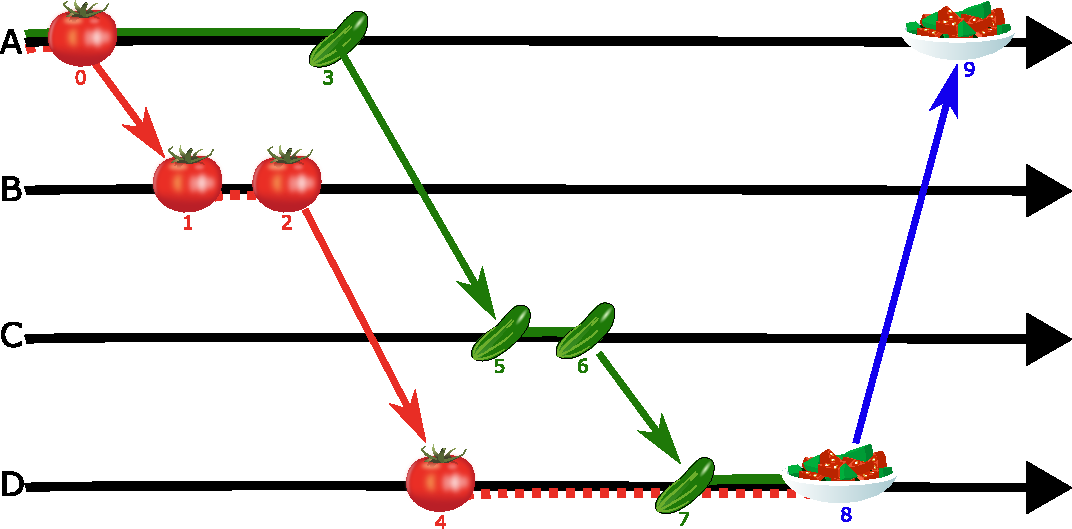
\includegraphics[width=\linewidth]{figs/salad_timeline.pdf}
    \caption{Timelines for 4 controllers, and resources for a virtual cooking application. Controllers are labeled with letters, and resources are labeled with numbers.}
    \label{fig:salad}
\end{figure}
Suppose four controllers ($A,B,C,$ and $D$) order transactions for a virtual cooking application (shown in~\cref{fig:salad}).
In the beginning, a tomato resource (0) and a cucumber resource (3) are on controller $A$.
The tomato resource transfers to $B$ (resource 0 is consumed, requiring whatever proofs are required to move a tomato, and resource 1 is created), and then, after some $B$-only transactions, it transfers to $D$ (resource 4).
Likewise, the cucumber resource transfers to $C$ and then to $D$ (resource 7).
On $D$, a transaction consumes both the tomato and cucumber resources to create a salad resource (resource 8). 
At this point, the salad resource's history depends on $A$, $B$, $C$, and $D$.
These are the affecting controllers of the salad's label.
If any of these controllers have been unsafe (as in~\cref{fig:saladfork}), there may be other resources elsewhere, claiming to represent the same tomato or cucumber that are supposedly part of this salad. 
The salad then transfers from $D$ to $A$, where the tomato and cucumber began.
Eventually, we want to allow $A$ to \emph{endorse} the salad's history, pledging not to endorse any alternative histories in which the cucumber or tomato did anything else, and removing the need to remember that $B$, $C$, or $D$ could have ``tainted'' the salad's history~\cite{dista}. 
They can be removed from the affecting controllers of the salad's label.

\section{Desiderata}
There are several properties we want our controllers and resource labels to have.
As a running example, consider~\cref{fig:saladfork}, a version of our salad example in which controller $B$ has forked into two traces: gray and black. 
Resource 10 (and therefore 11) has a \emph{conflicting} history with resource 2 (and therefore, 4, 8, and 9).


\subsection{Causal Resource History (CRH)}
We begin with a weak but relatively simple to maintain property: causally consistent resource history, or \emph{Causal Resource History (CRH)}~\cite{causal}.
A resource with CRH was created in a valid\footnote{\cite{resource} defines a ``valid'' transaction as not using an input that's already been consumed.
Here, as we lack global time, we require only that a transaction's inputs have not been consumed by a transaction in its \textit{causal} past.}
transaction, whose inputs were resources with CRH. 
This property is relatively easy to prove with recursive zero knowledge proofs (compared with some stricter properties we'll get to later)~\cite{nova}.
In general, in order to maintain CRH, a resource should carry a (recursive) proof that it was created in a valid transaction, the inputs of which had CRH proofs. 
In fact, CRH can be implemented in resource logics.

This property is not perfect: it still permits histories we might want to call \emph{inconsistent}, including double-consumes.
For example, in~\cref{fig:saladfork}, any future resource that depends on resources 9 and 11 (so, something constructed by consuming the salad and the tomato), would have a history in which the same tomato (which started as resource 0), is consumed twice, but would still have CRH.



\begin{figure*}
    \centering
    \centerline{
    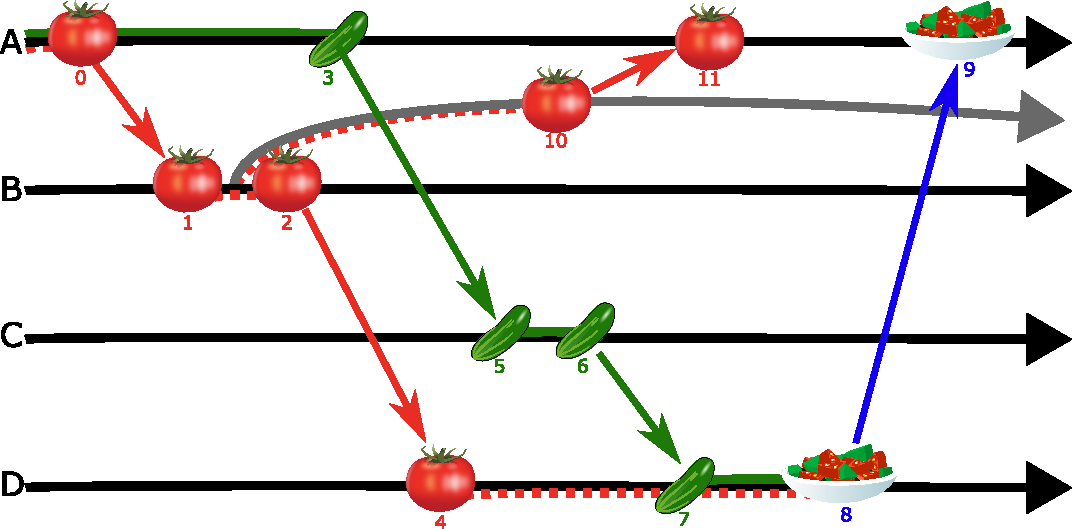
\includegraphics[width=0.85\linewidth]{figs/salad_timeline_fork.pdf}
    }
    \caption{Controller $B$ has forked into two timelines (gray and black).
             Resources 10 and 11 \emph{conflict} with resources 2, 4, 8, and 9.}
    \label{fig:saladfork}
\end{figure*}

\subsection{Serializable Resource History (SRH)}
Here we define what we consider \emph{consistent}: each resource (individually) reflects some fully serializable history featuring only correct atomic transactions (and no forks)~\cite{serializability}. 
Equivalently, in the resource's history, all transactions are valid, and no resource is used as an input for a transaction after it has been consumed. 
In our~\cref{fig:saladfork} example, resources 11 and 9 individually have SRH, but they cannot both appear in the history of any future resource with SRH (no one can consume both as an input in some transaction).
Alternatively, you could not combine money from both sides of the double-spend for one big purchase.
SRH can be easily generalized to a group of resources by imagining a new resource that depends on all of the resources in the group, and checking if it has SRH.

Maintaining SRH requires some kind of mechanism for checking if two resources can both be part of some future resource's history. 
Effectively, any such mechanism checks for forks, and can be used to filter for resources that have SRH.

%If a resource is part of\footnote{\emph{is part of} in what sense part of ???} a consistent controller state, then it must have a consistent resource history. 
%Likewise, if some resource's ancestors include all the resources on a controller, and that resource has a consistent resource history, then that controller has a consistent controller state.\footnote{something to understand about \emph{controller state}, best with an example of some specific paradigmatic type of controller state}

In~\cref{sec:resourcevectorclocks}, we detail a technique for maintaining SRH for all resources, but it can require very expensive computation and requires each resource to carry an ever-growing set of controllers in its label. 
Instead, we allow users to introduce a little trust into the system, and dramatically improve day-to-day operations.
We will detail techniques for checking SRH while using our technique, but each check can require a lot of information.

\subsection{Consistent Controller Label (CCL)}
% ICS: unclear how this sentence was supposed to help here: In general, a safe controller never uses a resource as a transaction input after it has been consumed: all inputs to any transaction it commits are created, unconsumed resources, and the transaction consumes (some subset of) those inputs, and creates new resources. 
The \emph{Consistent Controller Labels}  property (CCL) requires that if some resource~$r$ does not have SRH, then it has an unsafe controller in the \textit{affecting controllers} set in its label.
With CRH, if a user \textit{trusts} that a resource's affecting controllers are all safe, they can be sure the resource has SRH. 

One easy way to maintain CCL would be to start with a system that maintains CRH, and label every resource with every controller involved in its history (affecting controllers). 
If all the controllers are safe, then the resource has SRH. 
For example, in~\cref{fig:saladfork}, resource 8's affecting controllers include $A$, $B$, $C$, and $D$.
However, we explore optimizations that allow removing unnecessary controllers from the affecting controllers set.
For instance, in~\cref{fig:saladfork}, $A$ can \emph{endorse} the history of resource 9, and remove $B$, $C$, and $D$ from its affecting controllers.
The key in this case is to ensure that any future resource that depends on both resource 9 and resource 11 \emph{will} include $B$ in its affecting controllers.
To accomplish this, we prevent $A$ from endorsing (and thus removing $B$ from) the history of both resource 9 and resource 11.

In~\cref{sec:consistentcontrollerstate}, we introduce Consistent Controller State (CCS), an even stronger property than SRH, along with a technique to maintain it, but we believe the inherent ``forks split the world'' drawbacks  make CCS too strong to be worth using.

\section{Controller DAGs with Endorsement: a Technique for CCL}
\label{sec:dagswithendorsement}
In this approach, we maintain CRH and CCL, with relatively little overhead.
% ICS: we don't really define what little overhead means here.
% It's easiest to see what we're talking about there in contrast to other techniques (now in the appendix)
% The problem is that presenting all those other techniques first takes space and time. 
Resource label size can be kept proportional to the number of cross-controller resource transfers in its history (in the worst case), but in the best case is much smaller.
Moving a resource between controllers is relatively cheap, requiring only few simple checks and a single endorsement (which can be done as two recursive ZKP checks).
Endorsements are not resource-specific, so they can be done opportunistically and their costs amortized. 

\subsection{Controller State}
We assume each controller has a unique \emph{controller id}.
We also assume that each controller's entire state (including accumulators for which resources it has created and consumed, and everything else) can be uniquely identified with a digest or hash called a \emph{state root}.
We have a notion of one state (or state root) being provably \emph{after} another state (or state root) if the ``later'' one is the result of a (possibly empty) sequence of valid state transitions (transactions) ordered by the state root's controller, starting with the ``earlier'' one. 
We can define provably \emph{before} similarly. 

\noindent Each controller's state includes (but is not limited to) the
data in~\Cref{tab:controllerstate}.

\begin{table*}
\centerline{
\begin{tabular}{|l|l|p{0.5\textwidth}|}\hline
\textbf{Field} & \textbf{Type} & \textbf{Description} \\\hline
halted & boolean & Is this a halting state? There are no valid transitions from halting states.\\\hline
endorsement & map: controller id $\rightarrow$ state root & state roots of other controllers this controller has (non-recursively) endorsed.\\\hline
sends & set of \emph{send} & represents outgoing resource transfers\\\hline
receives & set of \emph{receives} & represents incoming resource transfers\\\hline
\end{tabular}}
\caption{Fields in a controller's state.}
\label{tab:controllerstate}
\end{table*}

\noindent The \textit{endorsement} map starts with every controller id mapping to genesis (whatever state root it must start with; this may be defined in the controller id itself).
There is one exception: the element for this controller's id is the state root for this state.
We also introduce a new type of transaction.
A controller id's endorsement element can be updated, given:
\begin{itemize}
    \item a proof that the new state root is provably after the old state root, and
    \item a proof that if the endorsed state root contains an endorsement for this controller, it endorsed a state root provably before this state (you can't endorse someone who has endorsed a fork of yourself).
\end{itemize}
Note that this update does \emph{not} require any kind of recursive update of controllers the endorsed controller has endorsed.

Next we discuss \emph{send} and \emph{receive} records.


\subsubsection{Send Records}
\begin{table*}
\centerline{
\begin{tabular}{|l|l|p{0.5\textwidth}|}\hline
\textbf{Field} & \textbf{Type} & \textbf{Description} \\\hline
id & send id & uniquely identifies this send record.\\\hline
resource & resource id & the resource sent.\\\hline
removable & boolean & defaults to false, true if this has no \emph{incoming}, or as a result of some activity that can only occur on this controller (e.g. minting a currency).\\\hline
updatable & boolean & defaults to true, set to false as part of endorsement-reduction.\\\hline
incoming & set of receive ids & the receive records on which this send depends.\\\hline
outgoing & set of controller ids & the controller(s) to which a resources were sent.\\\hline
\end{tabular}}
\caption{Fields of a \emph{send} record.}
\label{tab:send}
\end{table*}

Each controller maintains a set of \emph{send} records, which are created each time a resource transfer from one controller to another begins. 
To initiate a transfer, a controller consumes the sent resource, and creates a similar resource with a different \emph{terminal} controller, as well as a corresponding \emph{send} record. 
Each \emph{send} record has an (immutable) unique \emph{send id}, as well as fields described in~\cref{tab:send}.
If the transferred resource has ancestors from another controller, the \emph{incoming} field reflects the events when ancestors came to this controller. 
Similarly, the \emph{outgoing} field represents the destination of the transfer. 
This can be updated as part of the reducing process~(\cref{sec:reducing}). 
If a send record's \emph{updatable} field is false, it becomes immutable: it can never change again.
This is used in observer graph reduction~(\cref{sec:reducing}).

A \emph{send} record represents a \emph{promise}: when one controller transfers a resource to another, it promises to accept those resources, or new resources created using those, in transfers back. 
Pending a review of the returned resources' history, these can be treated just like resources created on the original sending controller. 
We describe this process in more detail in~\cref{sec:reducing}. 

\subsubsection{Receive Records}
\begin{table*}
\centerline{
\begin{tabular}{|l|l|p{0.5\textwidth}|}\hline
\textbf{Field} & \textbf{Type} & \textbf{Description} \\\hline
id & receive id & uniquely identifies this receive record.\\\hline
resource & resource id & the resource sent.\\\hline
incoming & set of send ids & non-empty set of send records on other controllers.\\\hline
live & set of resource ids & the created (and not consumed) resources on this controller which depend on this receive.\\\hline
outgoing & set of send ids & the sends on this controller created when recources dependent on this receive were sent elsewhere.\\\hline
\end{tabular}}
\caption{Fields of a \emph{receive} record.}
\label{tab:receive}
\end{table*}
Each controller also maintains a set of \emph{receive} records, which are created each time a transfer from one controller to another completes.
Note that a resource cannot be received twice: no state can contain two receives with the same \emph{id} or the same \emph{resource}. 
To receive a transfer, a controller creates a receive record, as well as a copy of the sent resource, whose terminal controller matches the destination controller.
Each \emph{receive} record has an (immutable) \emph{receive id}, as well as fields described in~\cref{tab:receive}.
A receive's \emph{incoming} field must feature at least one send, and all  on other controllers: these are the sends which this receive received. 


In a safe controller's state, each send in a receive's outgoing field should feature the receive in its incoming field. 

Note that send and receive records can be encoded as resources (with sufficiently precise resource logics). 
For our purposes, it is useful to discuss them as mutable records, even if they are implemented as resources ``under the hood.''



% Some invariants:
% \begin{itemize}
%   \item if a send and receive are on the same (safe) controller, then the send should reference the receive iff the receive references the send. 
%   \item A receive must reference at least one send on another controller.
%   \item If a send (on a safe controller) references a receive on another (safe) controller, that receive references that send. 
% \end{itemize}






% \noindent Each controller's state includes (but is not limited to) the
% data in~\Cref{tab:controllerstate}.
% 
% \begin{table*}
% \centerline{
% \begin{tabular}{|l|l|p{0.5\textwidth}|}\hline
% \textbf{Field} & \textbf{Type} & \textbf{Description} \\\hline
% halted & boolean & Is this a halting state? There are no valid transitions from halting states.\\\hline
% endorsement & map: controller id $\rightarrow$ state root & state roots of other controllers this controller has (non-recursively) endorsed.\\\hline
% \end{tabular}}
% \caption{Fields in a controller's state.}
% \label{tab:controllerstate}
% \end{table*}
% 
% \noindent The \textit{endorsement} map starts with every controller id mapping to genesis (whatever state root it must start with; this may be defined in the controller id itself).
% There is one exception: the element for this controller's id is the state root for this state.
% We also introduce a new type of transaction.
% A controller id's endorsement element can be updated, given:
% \begin{itemize}
%     \item a proof that the new state root is provably after the old state root, and
%     \item a proof that if the endorsed state root contains an endorsement for this controller, it endorsed a state root provably before this state (you can't endorse someone who has endorsed a fork of yourself).
% \end{itemize}
% Note that this update does \emph{not} require any kind of recursive update of controllers the endorsed controller has endorsed.

\subsection{Resource Controller Labels}
Each resource features a label with information about controllers that can or have affected it.
The label includes a DAG representing controllers who have affected the history of this resource.
Each \textit{node} of this DAG includes:
\begin{itemize}
\item a \emph{controller id}
\item a \emph{send id} representing when an ancestor of this resource was transferred out of this controller. 
\item a \emph{state root} for this controller, after (or equal to) the state when the \emph{send} was created.
\end{itemize}
For each edge in the DAG $s\rightarrow s^\prime$, there must be a receive id $r\in s.incoming$ such there is or was a corresponding receive record $r$ with $s^\prime \in r.incoming$. 
(here we abuse notation and use $r$ for both the receive id and the corresponding receive record.)
Without reductions~\cref{sec:reducing}, the DAG has an edge whenever there is such an $r$.
In this way, the controller DAG reflects (some of the) history of the resource. 

% Some invariants:
% \begin{itemize}
%   \item Each receive in the node should refer to at least one send in the node.
%   \item For each send in the node that refers to a receive in the node, that receive should in turn refer to that send. 
%   \item The state root should prove a valid sequence of transactions that created these sends and receives, and the state root should be before a root endorsed by the terminal controller
% \end{itemize}


% the fields
% in~\Cref{tab:resourcelabel}.
The set of all controllers from all the nodes of this DAG are the resource's \emph{affecting controllers}.


% \begin{table*}
% \centerline{
% \begin{tabular}{|l|l|p{0.55\textwidth}|}\hline
% \textbf{Field} & \textbf{Type} & \textbf{Description} \\\hline
% controller & controller id & a controller who affected this resource's history \\\hline
% state & state root & a state root from this controller \textit{after} (or equal to) the state resulting form the transaction that affected this resource's history \\\hline
% removable & boolean & If this resource (or some part of its history) the result of a transaction that could \textit{only} have run on this controller, or would not be able to run on arbitrary controllers, then this must be false.\\\hline
% reducing & $\bot$ or $\an{\textrm{controller id, state root}}$ & Are we in the process or removing this node from this controller DAG? (described below)\\\hline
% \end{tabular}}
% \caption{Fields in a resource controller label.}
% \label{tab:resourcelabel}
% \end{table*}


\noindent Each resource label also includes the fields
in~\cref{tab:resourcelabel2}.
% When discussing our~\cref{fig:saladfork} example, we write nodes as, for example, $A@11$, to denote controller $A$ with the state root it had just after creating resource 11.

\begin{table*}
\centerline{
\begin{tabular}{|l|l|p{0.5\textwidth}|}\hline
\textbf{Field} & \textbf{Type} & \textbf{Description} \\\hline
creating & controller id & which controller determines if this resource has been created?\\\hline
terminal & controller id & which controller determines if this resource has been consumed?\\\hline
backup & list of controller ids & If the terminal controller halts, who will be the new terminal controller? If that controller has halted, who will be the new terminal controller? and so on\dots\\\hline
receives & set of receive ids & the receive records (on the terminal controller) on which this resource depends.\\\hline
\end{tabular}}
\caption{Fields in a resource label.}
\label{tab:resourcelabel2}
\end{table*}


\subsection{Creating a resource}
A transaction must use as inputs resources with the same terminal controller: the controller that orders the transaction. 
The terminal controller's state determines if any of the input resources have been consumed (which would make the transaction invalid).
To determine if all the input resources have in fact been created, one must check whether the creating controller of the resource has created it. 
To ensure CRH, any resource with a creating controller other than the terminal controller requires a corresponding receive record to prove it has been created (see Transfers below).

A created resource can \textit{depend} on input resources, meaning the new resource's history includes those input resources, and their histories. 
In general, it is safe for a created resource to depend on all the input resources used in proofs of the resource's logic; this would work for very general applications.
However, we might allow resource logics to specify a subset of the input resources on which they depend. 
We might imagine a UTXO-style currency application~\cite{citation-needed} which tracks only input resources of the same currency as dependencies: anything which was necessary to authorize a ``spend'' isn't considered part of the history of the currency resource.

The resource's creating id is the id of the controller ordering the transaction that created it: this matches the terminal id of all the input resources.
If the resource's terminal id is another controller, this is a \emph{transfer}: the transaction must also produce a corresponding \emph{send} record. 
The resource has ``transferred'' to a different controller from its ancestors. 

Each resource's controller DAG includes the union of the controller DAGs of the input resources on which it depends.
If this is a transfer, then the DAG also includes a node for the new send record, and an edge from each sink of the input resource's DAGs to the new node.

Each resource's \emph{receives} field is the union of the \emph{receives} field of all of its dependencies, or for dependencies created on another controller, the corresponding receive record.
Each time a resource is created, it must be added to the \emph{live} set of each receive in its \emph{receives} field.
Likewise, each time a resource is consumed, it must be removed from the \emph{live} set of each receive in its \emph{receives} field. 

\subsubsection{Transfers}
In order to create a resource on one controller and consume it on another, there are several steps.
First, in a transaction on the sending controller:
\begin{itemize}
\item Create a new send id
\item Create the ``sent'' resource: it must have a new unique controller DAG sink: this send id. Do not add this resource to any receive record's \emph{live} field. 
\item add this send id to the \emph{outgoing} field of all the receives in the resource's \emph{receives} field.
\item Create a new send record with this new send id, referencing this resource, with \emph{incoming} set to the union of all of the receives of the dependencies. 
\end{itemize}
Second, on the receiving controller:
\begin{itemize}
  \item Endorse a state root from the sending controller whose corresponding state features the send record and the sent resource.
  \item Create a receive record  with a unique id, empty outgoing, a live set containing only the sent resource, and an \emph{incoming} field contianing only the send id.
        Future transactions can now consume the resource, and new resources which depend on it must put this receive record in their \emph{receives} field. 
\end{itemize}

For example, in~\cref{fig:salad}, In order the first transfer (resource 0 on $A$ to resource 1 on $B$), would require creating a send record $s_0$ on $A$, and a receive record $r_1$ on $B$, with $r_1.incoming=\cb{s_0}$.
Any subsequent resources representing the tomato would appear in $r_1.live$, until they are consumed.
Eventually, transferring resource 2 to $B$ creates a new send record, $s_2$ on $B$, and $r_1.outgoing$ must include $s_2$.
We illustrate the resulting state of affairs in~\cref{fig:start}.
Resource 4, then, with a history that depends on 2 sends, would have a Controller DAG: $A:s_0 \rightarrow B:s_2$, and terminal controller $C$. 


As a more in depth example, we draw the controller DAG for resource 9, with $s_n$ as the send record for sending resource $n$:

\begin{center}
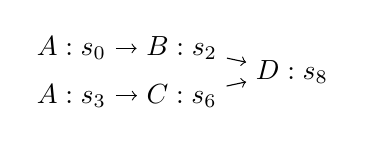
\begin{tikzpicture}
%\node (from) at (0,2) {from:};
%% nodes
\node (FA0) at (1,2.3) {$A:s_0$};
\node (FB2) at (2.4,2.3) {$B:s_2$};
\node (FA3) at (1,1.7) {$A:s_3$};
\node (FC6) at (2.4,1.7) {$C:s_6$};
\node (FD8) at (3.8,2) {$D:s_8$};
%%% edges
\draw[->] (FA0) -- (FB2);
\draw[->] (FB2) -- (FD8);
\draw[->] (FA3) -- (FC6);
\draw[->] (FC6) -- (FD8);

% \node(to) at (0,0) {to:};
% %% nodes
% \node (A) at (1,0) {$A@3$};
% \node (C) at (2.4,0.3) {$C@6$};
% \node (B) at (2.4,-0.3) {$B@2$};
% \node (D) at (3.8,0) {$D@8$};
% \node (A9) at (5.2,0) {$A@9$};
% %%% edges
% \draw[->] (A) -- (C);
% \draw[->] (A) -- (B);
% \draw[->] (B) -- (D);
% \draw[->] (C) -- (D);
% \draw[->] (D) -- (A9);
\end{tikzpicture}
\end{center}
Note that, since they have no \emph{incoming}, $s_0$ and $s_3$ have \emph{removable}=false.


\subsection{Reducing a Controller DAG}
\label{sec:reducing}

\subsubsection{Endorsement}
We can use the controller's endorsement map to remove unnecessary elements from a resource's controller DAG.
The idea is that if a resource's history involves moving to some intermediate controller, doing some transactions, and then moving on, the intermediate controller is \textit{arbitrary}: as long as other controllers are willing to check the part of the history done on the intermediate controller, they can claim they ``may as well have'' done those state changes themselves, and remove the intermediate controller.
This kind of endorsement-based DAG reduction generalizes IBC and ICS20's \emph{unwrapping} \cite{wrapped,ibc,ics20}.
In our~\cref{fig:saladfork} example, $A$ could endorse $C$, $D$, and (one fork of) $B$, and then reduce resource 9's controller DAG to just nodes with controller $A$.
The challenge is to do this in a way that provably maintains CCL. 
We would not want to allow resource 11 to end up with a DAG that doesn't contain $B$, or someone could consume resources 9 and 11 to create a new resource that doesn't have SRH (it contains a double-consume of a tomato), and also doesn't have $B$ in its controller DAG: that would violate CCL.
There are a number of subtleties here, so we start with some definitions.

\begin{definition}[Endorsement]
A controller $A$ \textit{endorses} a state root $R$ if $A$'s endorsement map element for $R$'s controller id is provably after (or equal to) $R$.
\end{definition}

\begin{definition}[Remove]
We \textit{remove} a node from a resource's controller DAG if we consume the resource, and create an identical one whose controller DAG is missing the node. 
Instead, the new resource's controller DAG has edges from all of the removed node's parents to all of the removed node's children.
\end{definition}
%Next we explore some ideas about how we might reduce a controller DAG using Endorsement. 


\begin{figure}[t]
\caption{Steps to generate a \emph{reduce proof} for $B$ in resource 4's DAG~(\cref{fig:salad}).
         The proof itself has a state root for $A$, $B$, and $D$, and shows they have the \emph{send} and \emph{receive} objects in \textbf{(d)}.}
\begin{subfigure}{.19\textwidth}
  \centering
  % include first image
  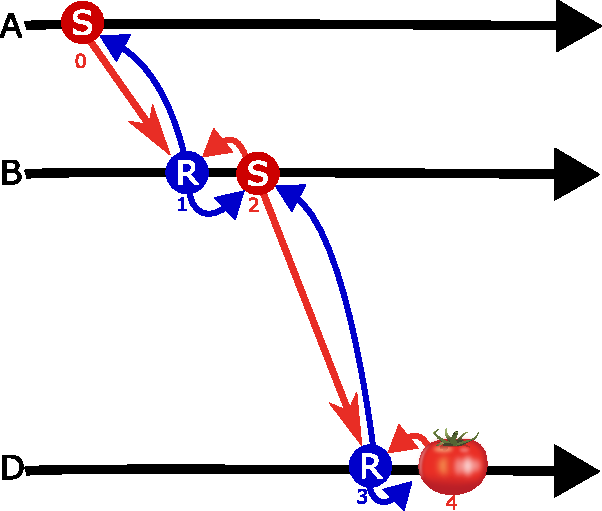
\includegraphics[width=\linewidth]{figs/sends_and_receives_start.pdf}  
  \caption{start}
  \label{fig:start}
\end{subfigure}
\begin{subfigure}{.19\textwidth}
  \centering
  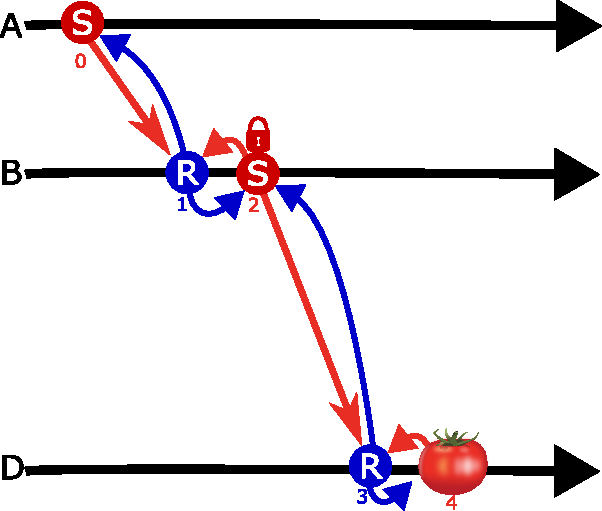
\includegraphics[width=\linewidth]{figs/sends_and_receives_send_lock.pdf}  
  \caption{updatable=false}
  \label{fig:updatable}
\end{subfigure}
\begin{subfigure}{.19\textwidth}
  \centering
  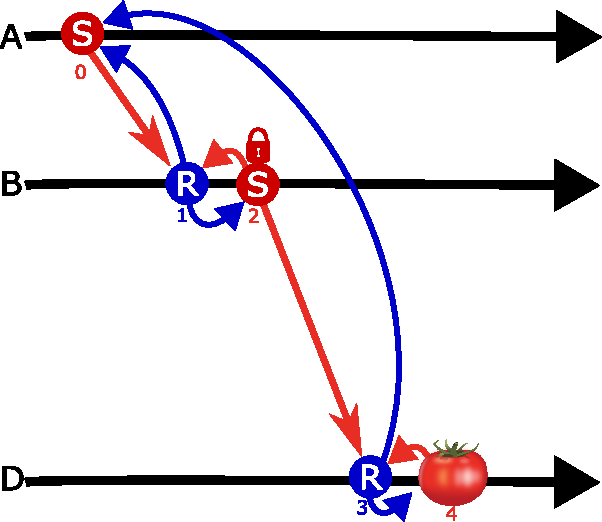
\includegraphics[width=\linewidth]{figs/sends_and_receives_proof_receive_redirect.pdf}  
  \caption{redirect receives}
  \label{fig:redirect}
\end{subfigure}
\begin{subfigure}{.19\textwidth}
  \centering
  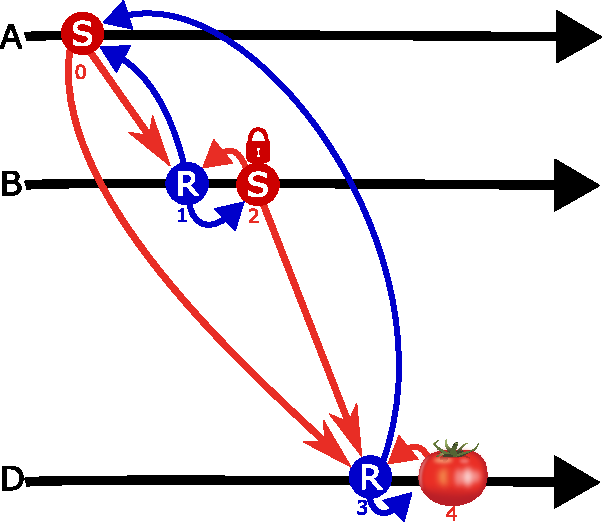
\includegraphics[width=\linewidth]{figs/sends_and_receives_proof.pdf}  
  \caption{update parents}
  \label{fig:update}
\end{subfigure}
\begin{subfigure}{.19\textwidth}
  \centering
  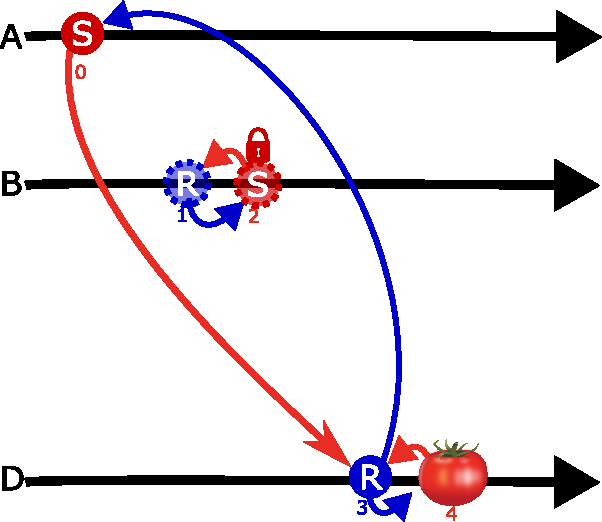
\includegraphics[width=\linewidth]{figs/sends_and_receives_remove_receive.pdf}  
  \caption{garbage collect}
  \label{fig:garbage}
\end{subfigure}
\label{fig:reduce-proof}
\end{figure}

\subsubsection{Reduce Proofs}
Before we can remove a node $n$, we require a \emph{reduce proof} for the send record in $n$.
Conceptually, a reduce proof shows that $n$'s parents and children have endorsed the history that happened on $n$'s controller, and agreed not to endorse any contradictory history.
Note that we can only create reduce proofs for sends with removable=true.
In ``promise'' terminology, wherein each send represents a promise to review and accept descendants of the sent resource, if $A$ promises to accept resources from $B$, and $B$ promises to accept resources from $C$, then with enough endorsement, we can collapse this to $A$ promising to accept resources directly from $C$. 
In taint tracking terminology, the controllers from $n$'s neighbors accept any responsibility for taint $n$'s controller might have caused, by reviewing the history of $n$'s send record. 


For a send record $s$, let $P\p s = \cb{s^\prime | r^\prime \in s.incoming \land s^\prime \in r^\prime.incoming}$ be the \emph{parents} of $s$.
These sends mark the boundary of $s$'s history on its own controller. 

For various reasons, it is convenient to define reduce proofs for sets of send records. 
Consider a set of sends $Y$ such that each send record has $removable=$true (which in turn implies that each has parents). 
We now detail the process of creating a reduce proof for $Y$. 

Let $X$ be the set of parents of sends in $Y$ which are not themselves in $Y$: $X = \cup_{y\in Y}P\p y / Y$.

Suppose a receive exists for every send in $Y$.
Let $Z$ contain a receive for each send in $Y$: $\forall y\in Y: \exists z\in Z : z.resource = y.resource$. 

Let the ancestors $a : Z \rightarrow 2^X$ of a receive record $z\in Z$ be the elements $x\in X$ such that there is a path (defined by \emph{incoming} field elements) from $z$ to $x$ in which all but the final send element ($x$) are in $Y$. 
These represent the boundary events that ``transitively affect'' $z$. 

Let $C: $ (set of send or receive $\rightarrow$ set of controller) be the function that maps a set of send or receive records to the controllers of those records, so $C\p Y$ is the set of controllers of the send records in $Y$. 

The steps to create a reduce proof for all the sends in $Y$ are below. 
In~\cref{fig:reduce-proof}, we illustrate this process with $Y=\cb{s_2}$, $X=\cb{s_0}$, and $Z=\cb{r_3}$. 
\begin{enumerate}
\item For eacy $y\in Y$, set $y.updatable$ to false~(\cref{fig:updatable}). This effectively prevents us from making a reduce proof for any of $y$'s ``neighbors'' (sends connected to the same receives as $y$) without making a reduce proof for $y$.
  Otherwise, we can get some very peculiar behavior where 2 resources with identical DAGs $A:s_0\rightarrow B:s_2 \rightarrow C:s_3 \rightarrow D:s_4$ can end up with DAGs $A:s_0 \rightarrow B:s_2 \rightarrow D:s_4$ and $A:s_0\rightarrow C:s_3 \rightarrow D:s_4$, which can cause problems for maintaining CCL.
\item Let $R_Y$ be the set of state roots of $C\p Y$ just after completing step 1.
\item For each controller in $C\p Z$:
  \begin{itemize}
    \item endorse all roots in $R_Y$.
    \item for each controller in $C\p X$, endorse a state root after all elements of $X$ were created. This essentially just recognizes that everything in $X$ has indeed occurred. 
    \item Update all receives $z \in Z$ by removing elements of $Y$ in $z.incoming$ and adding all elements of $a\p z$ to $z.incoming$~(\cref{fig:redirect}).
      Effectively, controller in $C\p Z$, having reviewd the history of $X\p Y$, accepts responsibility for the history (from $X$ onward) of the resources received.
  \end{itemize}
\item let $R_Z$ be the set of state roots of $C_Z$ just after completing step 3.
\item For each controller in $c \in C_X$:
  \begin{itemize}
     \item endorse $R_Y$ and $R_Z$.
     \item update all elements $x\in X$ to include outgoing references to the receives $Z$ \emph{after} $Y$:  $C\p z \in x.outgoing$ if $\exists z \in Z : c \in z.incoming$~(\cref{fig:update}). 
  \end{itemize}
\item The \emph{reduce proof} for each $y\in Y$ is a collection of state roots from all the controllers in $C\p X, C\p Y$, and $C\p Z$, with proofs that the above steps have happened.
      These proofs show that $\forall y\in Y: y.updatable$=false, all $z\in Z$ now have \emph{incoming} sends from $X$, and all $x\in X$ have been updated to refer to $C\p Z$ where appropriate. 
\end{enumerate}

Once enough reduce proofs have been generated, we can even garbage collect some send and receive records~(\cref{fig:garbage}). 
Specifically, when a send record $s_0$ has a controller $B$ in its \emph{outgoing} field, but all a receive records $r_1$ on $B$ receiving $s_0$ have an empty \emph{live} field, and there are reduce proofs for all the sends \emph{$r_1$.outgoing}, (and $B$ has endorsed state roots proving this is the case) we can remove $B$ from the $s_0$\emph{.outgoing}. 

Once all a receive record's incoming sends have removed that receive record's controller from their outgoing fields (and the receive record's controller has endorsed state roots that prove this), we can garbage collect the receive record: it will no longer be used. 
Once all of a send record's \emph{incoming} receive records are garbage collected (if the send record has \emph{removable}=true), we know that send will no longer be used, and can garbage collect it.

For liveness, reduce proofs should remain available indefinitely unless there is a way to prove that every resource with the send record in its controller DAG has been consumed. 
However, they do not need to be stored on any particular controller. 
We leave reduce proof distribution to future work. 

\subsubsection{Removing a Node from a Controller DAG}
For any transaction that creates a resource $r$ with a node $n$ in its controller DAG, removing $n$ requries a reduce proof for $n.send$.
First, $r$'s terminal controller must endorse all the state roots in the proof.
Then each node in $r$'s controller DAG must update its state root to whichever is provably after the other: the state root it currently has or the state root with the same controller in the proof. 
(If there is a state root with the same controller in the proof, but neither is provably after the other, this remove operation is not valid.)
Then it can remove $n$ from the controller DAG, and add edges from all of $n$'s parents to all of $n$'s children. 
For example, given a reduce proof for $s_2$, we could reduce the controller DAG of resource 9 (\cref{fig:saladfork}) from:

\begin{center}
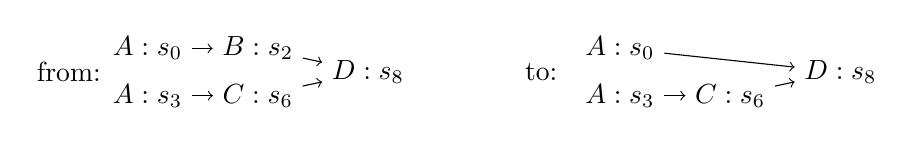
\begin{tikzpicture}
\node (from) at (0,2) {from:};
%% nodes
\node (FA0) at (1,2.3) {$A:s_0$};
\node (FB2) at (2.4,2.3) {$B:s_2$};
\node (FA3) at (1,1.7) {$A:s_3$};
\node (FC6) at (2.4,1.7) {$C:s_6$};
\node (FD8) at (3.8,2) {$D:s_8$};
%%% edges
\draw[->] (FA0) -- (FB2);
\draw[->] (FB2) -- (FD8);
\draw[->] (FA3) -- (FC6);
\draw[->] (FC6) -- (FD8);

 \node(to) at (6,2) {to:};
%% nodes
\node (FA0) at (7,2.3) {$A:s_0$};
\node (FA3) at (7,1.7) {$A:s_3$};
\node (FC6) at (8.4,1.7) {$C:s_6$};
\node (FD8) at (9.8,2) {$D:s_8$};
%%% edges
\draw[->] (FA0) -- (FD8);
\draw[->] (FA3) -- (FC6);
\draw[->] (FC6) -- (FD8);
\end{tikzpicture}
\end{center}
With enough reduce proofs, we could eventually reduce it to just $A:s_0$ and $A:s_3$ (and no edges).
Note that, since they have no \emph{incoming}, $s_0$ and $s_3$ have \emph{removable}=false, so they will never have a reduce proof.









\begin{theorem}[Reduction preserves CCL]
    If a safe controller creates a resource $r$, and valid transactions must follow the ``Creating a Resource'', endorsement, and ``Removing a Node from a Controller DAG'' procedures above, then $r$ has CCL.
\end{theorem}
\begin{proof}
First, we note that all resources created on safe controllers have CRH: safe controllers only create resources through valid transactions with inputs that have CRH, and only accept transferred resources after they have endorsed their history, proving the transferred resources have CRH. 

Consider $S$, the graph of send objects in the most recent state of all safe controllers, and all the most recent states of all forks of unsafe controllers. 
We define directed edges of $S$ using $P$: each send references any send which has \emph{ever been} its parent (an \emph{incoming} send of an \emph{incoming} receive).

All paths through $r$'s controllers DAG correspond to a path through $S$.
Some of the sends in that path may have reduce proofs, so there may be shorter paths.

Either $r$ has an unsafe controller in its DAG or it does not.
If $r$ has an unsafe controller in its DAG, then $r$ has CCL. 
Hereafter we consider the case where $r$'s dag is entirely safe. 

Either $r$ has SRH or it does not.
If $r$ has SRH, then $r$ has CCL. 
Hereafter we consider the case where $r$'s dag is entirely safe but $r$ does not have SRH.

Given that $r$ has CRH, lack of SRH means there is a fork in $r$'s history.
Some unsafe controller, which we will call $C$, created 2 contradictory \emph{send}s $s_1$ and $s_2$, which share an \emph{incoming} element, but neither of which is provably after the other.
If we consider all the transactions in $r$'s history in some serialized order, and consider the set of all sends in all (unconsumed) resources' controller DAGs, we show that no transaction can remove the last element of the last pair of contradictory sends. 

Specifically, suppose that $r$'s ancestor $a$ wishes to remove the last element $s_2$ of a contradictory pair of sends from unsafe controller $C$.
These sends share an \emph{incoming} element and therefore an ancestor send $s_0$ on another controller, which we'll call $B$. 
Without loss of generality, $s_0$ has $updatable$=false, since without an updatable ancestor, $B$ cannot be removed.
Therefore, $B:s_0$ has not yet been removed from $a$'s controller DAG.
$B$ cannot endorse both contradictory sends and add them to $s_0$ without forking and creating two contradictory versions of $s_0$.
Thus it is impossible to remove the last element of the last contradictory pair. 
Therefore, if $r$ does not have SRH, it has an unsafe controller in its DAG (and thus its affecting controllers). 
Thus CCL is guaranteed.

\end{proof}

\paragraph{Moving and Reducing Together}
It is possible to move a resource to another controller and remove the sender together. 
Specifically, the send is marked \emph{updatable}=true as soon as its created, and the receive updates its \emph{incoming} field immediately. 
With one transaction from the parents of the send, the received resource could remove the send the first time it's used. 

This is useful when, for example, some state has been temporarily moved from a base chain to a side chain, and the side chain wants to move it back to the base chain.
The side chain would condense all its nodes on the controller graph to a single node, and set that node's reducing field. 
The base chain could then endorse the side chain, and remove the side chain from the resource's controller DAG. 


\subsubsection{Removing a Halted Controller}
Controller states carry a boolean \textit{halted} flag, which defaults to false. 
At any time, changing this flag to true is a valid transition.
All transitions must be ordered / decided by the controller, so this transition would represent the controller deciding to halt. 
There are no valid state transitions starting with a state featuring a halted flag set to true. 
In effect, a \emph{halt} transaction creates a send for every unconsumed resource with \emph{outgoing} set to the resource's backup controller, and \emph{updatable} set to false.
A halted controller can also be said to have a receive record for every resource sent to it, followed immediately by a send. 

A connected sub-DAG (of a controller DAG) consisting entirely of halted controllers can be removed if all of the sub-DAG's children endorse every node in the sub-DAG, and all of the sub-DAG's parents endorse every element of the sub-DAG, and all of the sub-DAG's children. 
We can be certain that the halted controllers will not endorse some contradictory send (unless the halted controllers have forked), since they are halted, and cannot endorse anything. 

\subsubsection{Backup Controllers}
If the terminal controller has halted, a backup controller (who has endorsed a halted state for the halted controller) can assume control of the resource with a receive record. 
In order to show the corresponding send has in effect happened, the backup controller must also show that any earlier controllers in the resource label's \textit{backup} field have halted \textit{without} receiving this resource. 
This allows resources to survive a halted controller. 

A good default backup controller list might be derived some kind of path ``up'' the controller DAG, representing a history of controllers who have recently affected this resource. 

\subsubsection{Emergency Override Condition (EOC)}
Controllers decide on an order of transactions.
Usually this decision is defined by some kind of signature or record of consensus proving that some computer or computers decided on some ordering.
In principle, not all decisions (not all transactions) require the same procedure.
In particular, we can add to a controller a special case that is only allowed to do the halt transition.
We call this the Emergency Override Condition (EOC). 
For example, this could be some kind of high-integrity (but slow) ``supervisor'' who is trusted to declare when a controller's consensus mechanism (e.g. a blockchain) is dead.
If an EOC incorrectly halts a controller, but that controller continues ordering, it has forked: mistaken EOCs make controllers \emph{unsafe}. 

This does mean there could be multiple controllers who differ only in their EOC, but are otherwise maintained by the same consensus or machine.
These are still distinct controllers.
These controllers would be trivially able to endorse each other frequently, making transferring resources between them very easy. 
We might even be able to do atomic transactions consuming resources from both, although we leave that to future work. 



\subsection{Checking SRH}
The protocol described does not guarantee SRH.
A violation can occur when one of the controllers in the DAG has forked.
In our~\cref{fig:saladfork} example, a transaction could create a new resource which depends on resources 9 and 11.
Its controller DAG would include the forked controller $B$ (preserving CCL), but its history would not be serializable, and in fact contains a double-consumed tomato.

This can happen even if the controller appears only once in the DAG: the ``other'' fork may have been endorsed and removed by some parent in the DAG.
The easiest way to verify SRH of a resource or set of resources is to get a recent state root from each of the controller ids in their controller DAGs (and creating controllers), as well as all of their corresponding endorsed state roots for all the controller ids in the DAGs (and creating controllers), and then prove that for each controller: the ``recent'' state root is provably after all of the endorsed state roots or state roots in the DAG.
This would prove that no one has endorsed any fork contrary to the state roots in the DAG, and so the history is consistent. 

To understand why this holds, consider that a node with no parents cannot be removed (its send must have \emph{removable}=false), and if a node with an honest parent has forked, both sides of the fork cannot be removed without the honest parent endorsing one side of the fork.
The honest parent then cannot be removed from the other side, as it cannot endorse the contradictory send.

To ensure this information is always available would require each resource to carry an awful lot of information.
This is another case where a little trust goes a long way: if you trust that all the controllers in a resource's controller DAG haven't forked, then CCL (with CRH) implies SRH.
If you want to check, you can, but it requires acquiring more data.











% \section{Optimizations}
% There are some optimizations that I think we will want to put in the ``State Structure'' report. 
% For example, structure nullifiers with expiration dates, so we don't have to remember them forever.
% Also, we could tructure commitments with hierarchical times, and maybe forget the finer-grained commitment roots after a while. 

% \section{Implementation in Typhon}
% I'm not sure if this goes in the report either

% Includes what kind of extra inputs Typhon agrees upon for each transaction candidate (e.g. timestamp), and how those connect to the underlying machine (e.g. deletion crieterion).

% How does Typhon implement ``signing'' a resource / state change exactly?
% In fact, how do we specifically implement each of the anoma resource machine shell and core things, and how do we perform each of the operations listed above?

\section{Future Work}
There are several directions for future work. 
For instance, although all the techniques we have found for preserving SRH are expensive~(\cref{sec:resourcevectorclocks}), we have not proven that preserving SRH is inherently expensive. 
There may yet be some technique that is satisfactory. 

Likewise, we have not proven that it is crucial for controllers to retain resource-specific records to allow endorsement-based reduction (e.g. sends and receives).
There are almost certainly ways to batch and amortize these costs.
Perhaps there is even a system that only requires endorsement maps, like \cref{sec:ancestral}, while preserving the local ``only neighbors in the controller DAG need to participate in a reduce operation'' property. 

Furthermore, we make no claims about data availability, which is crucial for liveness.
Despite ordering transactions, controllers do not necessarily need to be able to calculate their state: zero-knowledge proofs can show that a transaction is valid without revealing much of what happened in it~\cite{nova,resource}.
We leave the difficult task of tracking what data needs to be available (including the current state of send and receive records), and to whom, to future work. 

 
\section{Concluding remarks}
We detail a technique for maintaining efficient controller labels with endorsement-based reduction.
Our technique keeps each transaction simple and inexpensive, and allows resources to carry relatively small labels, while simultaneously ensuring Causal Resource Histories and Consistent Controller Labels.
Fully Serializable Resource History remains check-able, although we show how a trust can improve performance, allowing CCL to be sufficient.
As part of a larger cross-domain architecture, our technique will allow more secure, more flexible cross-domain applications.




%%
%% Bibliography
%%
%% Please use bibtex, 
\bibliography{refs}

\appendix


\section{Resource Vector Clocks: a Technique for SRH}
\label{sec:resourcevectorclocks}
One approach to maintain SRH (no ``double-consumes" in the history of one resource) would be for each resource label to carry a \textit{vector-clock}: a map from controller ids to state roots. 
Resource labels also designate a creating controller (which must be in the vector-clock) and a terminal controller.
The ``affecting controllers'' in this technique are the keys of the vector-clock.

When a transaction creates a new resource, the new resource's vector-clock must feature all the controllers from all of the input resources' vector clocks, each mapped to a state root that is provably after (or equal to) the corresponding state roots from each of the input resources. 
This ensures the history of each resource cannot include a fork from any controller. 
The state root for the controller creating the resource must be that controller's current state root. 

\subsection{Problem: Cost}
Every transaction now has to do ``state root is after'' proofs for an unlimited number of controllers.

\subsection{Problem: Can't Remove Controllers}
There is no ``endorse'' mechanism that would allow a controller that appears in an ancestor to be absent from a descendant's vector-clock. 
This could lead to very large vector clocks in every resource, which result in lots of proofs with each transaction.

A fairly common pattern in the blockchain industry is to transfer resources from a more trustworthy ``base chain'' to a ``side-chain,'' or ``L2'' chain, do some transactions, and then transfer them back to the base chain, which somehow ``endorses'' the side-chain changes, so \textit{it doesn't matter where they happened}. 
Fundamentally, such an endorsement technique requires that the ``base chain'' remembers what it has endorsed, and doesn't endorse any conflicting histories. 
We have not encoded this in our vector clock model.
Furthermore, it is difficult to add: it is not clear which controllers should be empowered to endorse and remove which other controllers. 




\section{Consistent Controller State: Even Stronger than SRH}
\label{sec:consistentcontrollerstate}
One property we might want would be for each correct controller's state (the set of resources it can use as input for valid transactions) to reflect some fully serializable history featuring only correct transactions (and no forks). 
In~\cref{fig:saladfork}, for instance, controllers $C$ and $D$ have Consistent Controller State.
This would mean that, for example, if another controller has forked and produced resources representing a double-spend, no correct controller's state will contain resources affected by ``both sides'' of this double-spend.
In~\cref{fig:saladfork}, controller $A$ does not maintain consistent controller state, because its state contains resources 11 and 9, which descend from conflicting sides of a fork ($B$).

Consistent controller state is equivalent to requiring that all the resources on a controller together have SRH.
Likewise, SRH would be equivalent to consistent controller state if each controller had only one resource.

The techniques we have found to maintain consistent controller state are incredibly strict, which is why we generally use weaker properties.

\subsection{Recursive Endorsement: a Technique for Consistent Controller State}
The idea with this technique is to have each controller fully \textit{endorse}, or check, the entire history of other controllers, including the history of controllers they've endorsed.
This ensures that the state each controller recognizes is fully consistent.

\subsubsection{Controller State}
Suppose that each controller has a unique \textit{controller id}.
Suppose also that each controller's entire state (including representations of resources created, consumed, and everything else) can be uniquely identified with a digest or hash called a \textit{state root}.
Each controller's state also includes a \textit{recursive endorsement map}, which is a map from \textit{controller id}s to \textit{state root}s.
Its entry for itself is, in effect, its own state root.
At any time, (as a valid transaction), it can update the entry for any set of controllers, provided:
\begin{itemize}
    \item the new state root for all the controllers is proven after the old state root for all the controllers (or genesis, if there isn't one)
    \item The new recursive endorsement map includes state roots for all the controllers in all the recursive endorsement maps of the controllers updated.
    \item For pairs of elements ($\left\langle C_a, R_a\right\rangle$, $\left\langle C_b, R_b\right\rangle$) in the recursive endorsement map, if $R_a$'s recursive endorsement map includes an entry $\left\langle C_b, R_b^\prime\right\rangle$, then $R_b$ is provably after $R_b^\prime$.
\end{itemize}
Basically, each update \textit{includes} a recursive history check for all the controllers on which it depends.
This makes recursive endorsement map updates \emph{much} more expensive than regular endorsement map updates~(\cref{sec:dagswithendorsement}).

\subsubsection{Resource Labels}
Each resource label only specifies a \textit{terminal controller} id, a \textit{creating controller} id, and a \textit{creating controller state root}.
The creating controller state root is the state of the controller just after creating  the resource.
One possible type of transaction consumes a resource, and replaces it with a similar resource featuring a different terminal controller id.
This represents ``transferring'' the resource to a different controller. 
This can be constrained by the resource logic. 

In general (not only for transfers), a resource cannot be used in a transaction unless:
\begin{itemize}
    \item the transaction is ordered and executed on the resource's terminal controller.
    \item the terminal controller's recursive endorsement map state root for the resource's creating controller is proven after (or equal to) the resource's creating controller state root.
    \item all resources created by this transaction have a creating controller equal to the terminal controller of the inputs. 
    \item all resources created by this transaction have a creating controller state root representing the state of the creating controller after this transaction.
\end{itemize}
In other words, a resource can't be used on a controller until its history is fully endorsed. 

The nice thing is that transactions using resources created on the terminal controller are cheap, and resources each carry a constant amount of information about their controllers: they do not have to carry a set of ``affecting controllers.''
A resource is ``as trustworthy'' as its creating controller, and any controller that has endorsed that creating controller's state root (equal to or after this resource).


\subsubsection{Problem: Forks Split the World}
Suppose controller $B$ forks, and $A$ updates its recursive endorsement vector with one side of the fork, and $D$ updates its recursive endorsement vector with the other side. 
(This is what would happen in our~\cref{fig:saladfork} example.)
This means that hereafter, any resources $A$ creates cannot be used on $D$, and vice-versa. 
(The~\cref{fig:saladfork} transfer of resource 8 on $D$ to resource 9 on $A$ would be impossible.)
In fact, all controllers (if they ever use any resource from $B$), divide into 2 groups (one for each side of the fork), which can never interact again. 

This problem doesn't happen (or is less bad) if we only have to preserve SRH, because transactions only depends on input resources' history, so, in our~\cref{fig:saladfork} example, the transfer of resource 8 on $D$ to resource 9 on $A$ would be ok.
Furthermore, resources on $A$ that weren't actually affected by anything after the $B$ fork could still transfer to $D$ (which they can't in consistent controller state). 


\section{Ancestral Endorsement Reduction}
\label{sec:ancestral}
In~\cref{sec:reducing}, we discuss a technique for removing nodes from the controller DAG that requires controllers to keep send and receive records, in addition to an endorsement map. 
This technique does not require such records.
Unfortunately, this technique is not \emph{local}: it involves participation from controllers beyond just the neighbors of the nodes to be removed, or the terminal controller.

Each resource's label contains a DAG of state roots.
The resource's affecting controllers are the controllers of all the state roots in its DAG.
Each created resource's DAG contains the DAGs from all of their dependencies, with a new state root as a sink, representing the state of the creating controller upon completion of this transaction. 
We also allow transactions to update any state root to a state root provably after the old one. 

We allow a transaction to remove a node from a resource DAG if:
\begin{itemize}
    \item the node has parents (it is not a source in the DAG)
    \item all of the node's ancestors endorse the node
\end{itemize}
This preserves CCL, because we cannot remove sources, and if a controller forks, its parent cannot endorse both sides of the fork (without forking themselves). 
Intuitively, if there is a double-spend, at least one side of the spend will never be able to remove all the forked controllers from its controller DAG. 

The problem is that this is very expensive. 
It involves activity from an arbitrarily large set of controllers for every removal. 
What's more, sources in the controller DAG essentially have to endorse every removal, so they can end up doing a lot of work (although this can be batched and amortized), with no way to offload that responsibility to anyone else. 
If, for example, a cryptocurrency issuer moves tokens to other controllers and then becomes inactive for a long time (perhaps because it doesn't want to issue new currency for a while), then none of those tokens can do any ancestral endorsement reduction during that time.

Unfortunately, resources cannot allow both Ancestral Endorsement Reduction and reduction as we've outlined above: we have not found a CCL-preserving system that does both.


\end{document}
